% Options for packages loaded elsewhere
\PassOptionsToPackage{unicode}{hyperref}
\PassOptionsToPackage{hyphens}{url}
\PassOptionsToPackage{dvipsnames,svgnames,x11names}{xcolor}
%
\documentclass[
  authoryear,
  preprint,
  1p,
  onecolumn]{elsarticle}

\usepackage{amsmath,amssymb}
\usepackage{iftex}
\ifPDFTeX
  \usepackage[T1]{fontenc}
  \usepackage[utf8]{inputenc}
  \usepackage{textcomp} % provide euro and other symbols
\else % if luatex or xetex
  \usepackage{unicode-math}
  \defaultfontfeatures{Scale=MatchLowercase}
  \defaultfontfeatures[\rmfamily]{Ligatures=TeX,Scale=1}
\fi
\usepackage{lmodern}
\ifPDFTeX\else  
    % xetex/luatex font selection
\fi
% Use upquote if available, for straight quotes in verbatim environments
\IfFileExists{upquote.sty}{\usepackage{upquote}}{}
\IfFileExists{microtype.sty}{% use microtype if available
  \usepackage[]{microtype}
  \UseMicrotypeSet[protrusion]{basicmath} % disable protrusion for tt fonts
}{}
\makeatletter
\@ifundefined{KOMAClassName}{% if non-KOMA class
  \IfFileExists{parskip.sty}{%
    \usepackage{parskip}
  }{% else
    \setlength{\parindent}{0pt}
    \setlength{\parskip}{6pt plus 2pt minus 1pt}}
}{% if KOMA class
  \KOMAoptions{parskip=half}}
\makeatother
\usepackage{xcolor}
\setlength{\emergencystretch}{3em} % prevent overfull lines
\setcounter{secnumdepth}{5}
% Make \paragraph and \subparagraph free-standing
\makeatletter
\ifx\paragraph\undefined\else
  \let\oldparagraph\paragraph
  \renewcommand{\paragraph}{
    \@ifstar
      \xxxParagraphStar
      \xxxParagraphNoStar
  }
  \newcommand{\xxxParagraphStar}[1]{\oldparagraph*{#1}\mbox{}}
  \newcommand{\xxxParagraphNoStar}[1]{\oldparagraph{#1}\mbox{}}
\fi
\ifx\subparagraph\undefined\else
  \let\oldsubparagraph\subparagraph
  \renewcommand{\subparagraph}{
    \@ifstar
      \xxxSubParagraphStar
      \xxxSubParagraphNoStar
  }
  \newcommand{\xxxSubParagraphStar}[1]{\oldsubparagraph*{#1}\mbox{}}
  \newcommand{\xxxSubParagraphNoStar}[1]{\oldsubparagraph{#1}\mbox{}}
\fi
\makeatother


\providecommand{\tightlist}{%
  \setlength{\itemsep}{0pt}\setlength{\parskip}{0pt}}\usepackage{longtable,booktabs,array}
\usepackage{calc} % for calculating minipage widths
% Correct order of tables after \paragraph or \subparagraph
\usepackage{etoolbox}
\makeatletter
\patchcmd\longtable{\par}{\if@noskipsec\mbox{}\fi\par}{}{}
\makeatother
% Allow footnotes in longtable head/foot
\IfFileExists{footnotehyper.sty}{\usepackage{footnotehyper}}{\usepackage{footnote}}
\makesavenoteenv{longtable}
\usepackage{graphicx}
\makeatletter
\def\maxwidth{\ifdim\Gin@nat@width>\linewidth\linewidth\else\Gin@nat@width\fi}
\def\maxheight{\ifdim\Gin@nat@height>\textheight\textheight\else\Gin@nat@height\fi}
\makeatother
% Scale images if necessary, so that they will not overflow the page
% margins by default, and it is still possible to overwrite the defaults
% using explicit options in \includegraphics[width, height, ...]{}
\setkeys{Gin}{width=\maxwidth,height=\maxheight,keepaspectratio}
% Set default figure placement to htbp
\makeatletter
\def\fps@figure{htbp}
\makeatother

\usepackage{booktabs}
\usepackage{longtable}
\usepackage{array}
\usepackage{multirow}
\usepackage{wrapfig}
\usepackage{float}
\usepackage{colortbl}
\usepackage{pdflscape}
\usepackage{tabu}
\usepackage{threeparttable}
\usepackage{threeparttablex}
\usepackage[normalem]{ulem}
\usepackage{makecell}
\usepackage{xcolor}
\usepackage[section]{placeins}
\usepackage{pdfcomment}
\usepackage{gb4e} \noautomath
\makeatletter
\@ifpackageloaded{caption}{}{\usepackage{caption}}
\AtBeginDocument{%
\ifdefined\contentsname
  \renewcommand*\contentsname{Table of contents}
\else
  \newcommand\contentsname{Table of contents}
\fi
\ifdefined\listfigurename
  \renewcommand*\listfigurename{List of Figures}
\else
  \newcommand\listfigurename{List of Figures}
\fi
\ifdefined\listtablename
  \renewcommand*\listtablename{List of Tables}
\else
  \newcommand\listtablename{List of Tables}
\fi
\ifdefined\figurename
  \renewcommand*\figurename{Figure}
\else
  \newcommand\figurename{Figure}
\fi
\ifdefined\tablename
  \renewcommand*\tablename{Table}
\else
  \newcommand\tablename{Table}
\fi
}
\@ifpackageloaded{float}{}{\usepackage{float}}
\floatstyle{ruled}
\@ifundefined{c@chapter}{\newfloat{codelisting}{h}{lop}}{\newfloat{codelisting}{h}{lop}[chapter]}
\floatname{codelisting}{Listing}
\newcommand*\listoflistings{\listof{codelisting}{List of Listings}}
\makeatother
\makeatletter
\makeatother
\makeatletter
\@ifpackageloaded{caption}{}{\usepackage{caption}}
\@ifpackageloaded{subcaption}{}{\usepackage{subcaption}}
\makeatother
\journal{None}

\ifLuaTeX
  \usepackage{selnolig}  % disable illegal ligatures
\fi
\usepackage[]{natbib}
\bibliographystyle{elsarticle-harv}
\usepackage{bookmark}

\IfFileExists{xurl.sty}{\usepackage{xurl}}{} % add URL line breaks if available
\urlstyle{same} % disable monospaced font for URLs
\hypersetup{
  pdftitle={The effects of frequency and predictability on the recognition of up in English verb+up collocations.},
  pdfauthor={Zachary Houghton; Jungah Lee; Casey Felton; Georgia Zellou; Emily Morgan},
  colorlinks=true,
  linkcolor={blue},
  filecolor={Maroon},
  citecolor={Blue},
  urlcolor={Blue},
  pdfcreator={LaTeX via pandoc}}


\setlength{\parindent}{6pt}
\begin{document}

\begin{frontmatter}
\title{The effects of frequency and predictability on the recognition of
\emph{up} in English verb+up collocations.}
\author[1]{Zachary Houghton%
%
}
 \ead{znhoughton@ucdavis.edu} 
\author[2]{Jungah Lee%
%
}

\author[1]{Casey Felton%
%
}

\author[1]{Georgia Zellou%
%
}

\author[1]{Emily Morgan%
%
}


\affiliation[1]{organization={University of California,
Davis},,postcodesep={}}
\affiliation[2]{organization={Chosun University},,postcodesep={}}

\cortext[cor1]{Corresponding author}





        
\begin{abstract}
The question of what items are stored in the lexicon is one that has
drawn a lot of attention in the last few decades, and while the general
consensus is that a lot more is stored than we previously realized, it
is still largely unclear what factors drive storage. For example, some
have argued that frequency drives storage, while others have posited
that predictability drives storage. Further, it is unclear what the
relationship between stored multi-word items and the representation of
each individual word is. For example, it is possible that stored items
fuse together, losing some amount of their internal structure. The
present paper examines both of these questions by looking at the
recognizability of the segment \emph{up} in English V+\emph{up} phrases.
We find that the time it takes to recognize \emph{up} decreases as
frequency or predictability increases, but increases once again for the
highest frequency or highest predictability items. Our results suggest
that frequency and predictability both drive storage, and that stored
items may lose some amount of their internal representation.
\end{abstract}





\end{frontmatter}
    

\section{Introduction}\label{introduction}

When a listener hears the phrase \emph{trick or treat}, do they process
it compositionally, processing each word individually before combining
them into a single parse? Or do they access a single holistically stored
representation of the phrase from memory? This question of to what
extent larger-than-word constructions can be stored and accessed
holistically is one that psycholinguists have been interested in for
quite some time
\citep[e.g.,][]{bybee2002, bybee2003, goldberg2003, nooteboom2002, stembergerFrequencyLexicalStorage1986, stemberger2004}.

Throughout the years different theories have argued for different
degrees of holistic storage, with two theories in particular dominating
the field. On one hand, Chomskyan theories
\citep[e.g.,][]{chomskyAspectsTheorySyntax1965, pinkerFutureTense2002}
have proposed that only necessary items (e.g., items that can't be
formed compositionally) are stored.\footnote{Although some theories
  \citep[e.g.,][]{pinkerFutureTense2002} have accepted that some very
  high-frequency items may be stored due to human memory, but these
  theories are much more conservative about what is stored compared to
  usage-based theories.} On the other hand, usage-based theories
\citep[e.g.,][]{bybee2003} have proposed that many items that could in
principle be formed compositionally can be stored under certain
usage-based conditions, such as frequency of use.

Traditional Chomskyan theories
\citep[e.g.,][]{chomskyAspectsTheorySyntax1965, pinkerFutureTense2002}
have argued that processing multi-word phrases is completely
compositional: each piece is accessed individually and then combined to
form the larger meaning. Some exceptions are reserved for idioms and
other outliers, which can't be formed compositionally. More
specifically, Chomskyan views of storage argue that whether an item is
stored is determined purely by the degree of compositionality. According
to these theories, if a multi-word expression can be composed from its
parts then there is no need to holistically store the expression, and
thus it is not stored holistically. For example since \emph{I don't
know} can be processed compositionally, it would be processed by
composing a representation from each of the individual words, \emph{I,
don't,} and \emph{know}. On the other hand, \emph{kicked the bucket}
would be stored holistically because there's very little relationship
between the meaning of the individual words and the meaning of the
expression (i.e., it's non-compositional).

Chomskyan theories of storage gained popularity partly because storage
was thought to be a valuable resource that was taken up only by units
that necessitated storage. This was perhaps influenced by the limited
storage space of sophisticated computers at the time. In recent times,
however, we've learned that the brain may have dramatically more space
for storage than we had previously realized, with an upper bound of
10\textsuperscript{8432} bits \citep{wang2003}. This is magnitudes
larger than any current estimate of how much storage language
requires.\footnote{Indeed, \citet{mollica2019} estimated that, in terms
  of linguistic information, humans store only somewhere between one
  million and ten million bits of information, meaning that even their
  upper estimate is well within the capacity of the brain.} Considering
this, it might not come as a surprise that there has been a rise in
support for usage-based theories of holistic storage over the past few
decades
\citep{kapatsinski2009, kapatsinski2018, stembergerFrequencyLexicalStorage1986, stemberger2004, morgan2016, bybee1999, bybee2001, bybee2002, bybee2003, baayenDutchInflectionRules2002, ambridgeStoredAbstractionsRadical2020, zangParafovealProcessingChinese2024}.

Usage-based theories posit that more than just non-compositional items
(e.g., multi-word expressions) may be stored holistically in the
lexicon, arguing that storage is driven by usage-based factors. For
example, factors like frequency or predictability of the phrase may
influence whether the phrase is stored holistically or not. According to
these theories, in addition to idioms and non-compositional items,
multi-word phrases such as \emph{I don't know} may also be stored
holistically if they are used frequently enough
\citep[e.g.,][]{ambridgeStoredAbstractionsRadical2020, kapatsinski2018, kapatsinski2009, hay2001, lee2015, arnon2010, stembergerFrequencyLexicalStorage1986, stemberger2004, morgan2016, tomasello2005}.

While it has become a dominant view in the field that at least some
multi-word items are stored, it remains unclear what exactly the size of
the units being stored is and, more so, what the factors driving storage
are. Further, if multi-word representations are stored holistically,
what are the consequences of this in terms of language processing?

\subsection{Evidence of Holistic
Storage}\label{evidence-of-holistic-storage}

There is no shortage of evidence for holistic multi-word storage
\citep[e.g.,][]{bybee1999, stembergerFrequencyLexicalStorage1986, stemberger2004, hay2001, christiansen2017, zwitserlood2018},
especially in the phonology literature. For example, \citet{bybee1999}
demonstrated that the word \emph{don't} is reduced to a larger extent in
the phrase \emph{I don't know} than in other phrases containing
\emph{don't}. In other words, the phrase \emph{I don't know} seems to
have its own mental representation. If it was the case that the
representation of \emph{don't} in \emph{I don't know} was the same as
the representation of \emph{don't} in other contexts, then one would
expect \emph{don't} to be equally reduced in both cases \citep[which is
contrary to the finding in][]{bybee1999}. Similarly, in Korean, certain
consonants undergo tensification when they occur after the future marker
-\emph{l}. The rate of this tensification is higher in high-frequency
phrases than low-frequency phrases, further suggesting that
high-frequency phrases may be stored holistically \citep{yi2002}.

In addition to the phonology literature, the Psycholinguistics
literature has also provided an abundance of evidence for multi-word
storage. For example, \citet{siyanova-chanturia2011} demonstrated that
binomial phrases (e.g., \emph{cat and dog}) are read faster in their
more frequent ordering than in their less frequent ordering. Further, in
a follow-up study, \citet{morgan2016} demonstrated that these ordering
preferences for frequent binomials are not due to abstract ordering
preferences (e.g., a preference for short words before long words), but
are rather driven by experience with the specific binomial (i.e., how
frequent each binomial ordering is), providing additional evidence that
frequent phrases are stored holistically.

Similarly, \citet{arnon2010} demonstrated that frequent multi-word
phrases are read faster than lower frequency multi-word phrases, even
after accounting for the frequency of the individual words. This
suggests that humans are sensitive to the frequencies of multi-word
phrases. Further, in language production humans are also sensitive to
the frequency of multi-word phrases. In a production study,
\citet{janssenPhraseFrequencyEffects2012} found that participants
produced frequent multi-word phrases faster than lower frequency
phrases, even after taking into account the frequencies of the
individual words.

Further, there is also evidence of multi-word storage from the learning
literature \citep{siegelman2015, bannardStoredWordSequences2008}. For
example, \citet{siegelman2015} demonstrated that learning is facilitated
by attending to the whole utterance, as opposed to attending to each
individual word. Specifically, they used an artificial language paradigm
to examine adult L2 learners' ability to learn grammatical gender. They
found that adults learn grammatical gender better when they are
presented with unsegmented utterances rather than segmented utterances.
In other words, attending to the entire utterance, rather than learning
to compose the utterance word-by-word, facilitated their learning. It
seems plausible that if the entire utterance is being attended to, then
participants may be learning (i.e., storing) the entire utterance
initially. Further, storing larger-than-word chunks may possibly be
facilitating the learning of grammatical gender in their study.

\subsection{What Drives Storage?}\label{what-drives-storage}

Despite the evidence of multi-word holistic storage, however, it is
still largely unclear what factors drive storage. Humans seem to be
sensitive to a variety of statistical information, including both
frequency \citep[e.g.,][]{bybee1999, maye2000, kapatsinski2009, lee2015}
and predictability \citep[e.g,][]{olejarczuk2018, ramscar2013}.

Traditionally, frequency has been assumed to be the driving factor
behind multi-word storage. Indeed, most of the examples of storage given
so far have been with respect to frequency. Perhaps the most famous
series of studies demonstrating this were conducted by Bybee
\citep{bybee1999, bybee2003, bybee2001}. In a series of studies, Bybee
and colleagues demonstrated that a variety of words are reduced more in
high-frequency contexts than low-frequency contexts \citep[additionally
see][ for further discussion of
this]{kapatsinskiHierarchicalInferenceSound2021}. For example, in
addition to the earlier examples, \emph{going to} can be reduced in the
frequent future marker, \emph{gonna}, but not in the less frequent verb
phrase construction describing motion \citep[e.g., *\emph{gonna the
store},][]{bybee2003}. This mirrors patterns we see on a word-level
(which for the most part must be stored). For example, the reduction of
vowels to schwa in English is more advanced in high-frequency words than
low-frequency words \citep{hooper1976, bybee2003}. In other words, for
both words and phrases, sound reduction advances more quickly as a
function of frequency (i.e., high frequency phrases and high frequency
words are both more reduced than their lower frequency counterparts).
While this is not surprising for words (which most theories posit have
separate representations), it is surprising for phrases which don't
necessarily have to be stored holistically.

On the other hand, predictability has not been directly examined much by
the Psycholinguistics literature within the context of holistic
multi-word storage
\citep[c.f.][]{odonnellFragmentGrammarsExploring2009, houghton2023does}.
One such study examining the role of predictability in holistic storage
was \citetext{\citealp{houghton2023does}; \citealp[which was an
extension of][]{staub2007}}. In their study, using the maze
task\footnote{In the maze task, participants are presented a sentence
  word-by-word. For each word in the sentence, they are presented with
  the target word and an ungrammatical distractor. Upon selecting the
  target word, the next word in the sentence is presented along with yet
  another ungrammatical distractor. The key measure is how long it takes
  for participants to select the target word.}
\citep{boyceMazeMadeEasy2020} the authors examined whether participants
were slower to select the first noun in high-predictability compound
nouns in locally implausible contexts (i.e., contexts where the first
noun in the compound is implausible but where the second noun eliminates
the implausibility; see the below sentences) relative to
high-predictability compound nouns in locally plausible contexts.

\begin{enumerate}
\def\labelenumi{\arabic{enumi}.}
\item
  \begin{description}
  \item[\textbf{High Predictability Plausible:}]
  ~~~~~~~~Jimmy spread out the peanut butter.
  \end{description}
\item
  \begin{description}
  \item[\textbf{High Predictability Implausible:}]
  ~~~~Jimmy picked up the peanut butter.
  \end{description}
\end{enumerate}

\noindent Note that in the implausible condition, the second noun always
eliminates the implausibility (i.e., \emph{spread out the peanut} is
implausible, but \emph{spread out the peanut butter} is not). If
high-predictability compound nouns are stored holistically, participants
may be able to access the full compound noun upon encountering the first
noun, thus overcoming the local implausibility effect (since the second
noun in the compound always eliminates the implausibility). The authors
found that the first noun in the compound nouns was selected slower in
the implausible condition than in the plausible condition.
Interestingly, this slowdown was roughly the same regardless of the
predictability of the compoud noun. That is, there was an increase in
reaction time for selecting the first noun in the compound in the
implausible condition (relative to the plausible condition) regardless
of the predictability of the second noun in the compound noun. Their
results suggest that either predictability doesn't drive the holistic
storage of compound nouns or that it doesn't facilitate processing in
this manner. However they noted that this may be a task effect, since
they used the maze task as opposed to an eye-tracking task.

Despite the lack of direct evidence of predictability in the role of
multi-word storage, however, predictability has been shown to play a
crucial role in learning
\citep{olejarczuk2018, ramscar2013, saffran1996}. For example,
\citet{olejarczuk2018} demonstrated that when learning new phonetic
categories, learners don't just pay attention to co-occurrence rates,
but actively try to predict upcoming sounds, suggesting that the
learning of phonetic categories is also driven by prediction (i.e., the
predictability of a given sound within a context). Further, in learning
new words, \citet{ramscar2013} demonstrated that children are sensitive
to how predictable a cue is of an outcome (e.g., a high-frequency cue
will be ignored if it isn't predictive of a specific outcome).
Additionally, word-segmentation (i.e., learning which segments in an
utterance are words) is also highly sensitive to predictability
\citep{saffran1996}. In their classic paper, \citet{saffran1996}
demonstrated that children keep track of transitional probabilities -- a
measurement of predictability -- to segment the speech stream. While
these are studies examining learning, not storage, the units that we
learn may likely be the units we store. If predictability drives what we
learn, it may also drive what we store.

Thus, the current literature presents strong evidence for the role of
frequency in the storage of multi-word phrases, as well as suggests the
possibility of a further influence of predictability. However, it
remains unclear to what extent each of these factors drives storage and
whether they interact at all with each other.

\subsection{Representation of Stored
Units}\label{representation-of-stored-units}

Given the evidence that a lot more may be stored than previously
thought, another important question to consider is what the internal
representations of these units is. Specifically, do the stored units
maintain their own internal representation with respect to their
component parts? For example, it is possible that the representation of
high-frequency phrases, such as \emph{pick up,} retains the
representations of the component parts \emph{pick} and \emph{up}
(Figure~\ref{fig-lossinternalstructure}). On the other hand, it is
possible that the phrase lacks internal representation of the component
parts, either because it was lost over time or because it was not
learned to begin with.

Indeed, there seems to be some evidence that multi-word phrases may not
have a fully intact internal structure with respect to their component
parts. For example, \citet{kapatsinski2009} demonstrated that in high
frequency V+\emph{up} constructions, it is harder to recognize the
segment \emph{up} (with respect to medium-frequency V+\emph{up}
constructions). This suggests that those items may have a holistic
representation that has lost some of its internal structure. In their
study, participants were given different auditory sentences and tasked
with pressing a button immediately if they heard the segment \emph{up}.
Interestingly, they found that recognizability of \emph{up} follows a
U-shaped pattern with respect to the frequency of the phrase. That is,
participants were slow to recognize \emph{up} in low frequency phrasal
verbs, but for medium-high frequency phrasal verbs they were quicker to
recognize \emph{up}. However, upon reaching the highest frequency words
participants once again grew slower to recognize \emph{up} (See
Figure~\ref{fig-kapatsinskiplot}). Though it's important to note that
the original paper does not take into account predictability. It's
unclear how to account for the increase in recognition time for the
highest frequency items if there is no loss of internal representation
of those items.

A visualization of what a stored representation with and without
internal structure may look like is presented in
Figure~\ref{fig-lossinternalstructure}. The left tree represents the
phrase \emph{pick up} stored with its internal structure still intact,
whereas the right tree represents \emph{pick up} stored without internal
structure. Note that both trees are examples of a holistically stored
representation. The key difference is whether the internal structure
remains intact in the holistic representation. The results from
\citet{kapatsinski2009} suggest that for high-frequency verb+\emph{up}
collocations, their representation may be more similar to the tree on
the right, since participants were slower to recognize \emph{up}. We
will revisit this point in the discussion section in more detail.

\begin{figure}

\centering{

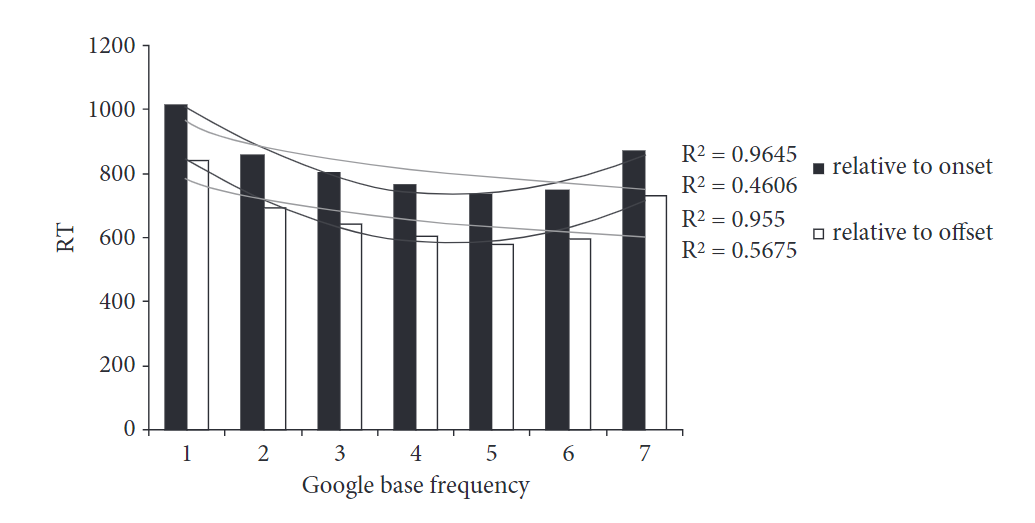
\includegraphics{Figures/kapatsinskiradicke_graph.png}

}

\caption{\label{fig-kapatsinskiplot}The U-shaped effect of the frequency
of verb+\emph{up} constructions on the speed with which \emph{up} is
detected, reproduced from \citet{kapatsinski2009}.}

\end{figure}%

\begin{figure}

\centering{

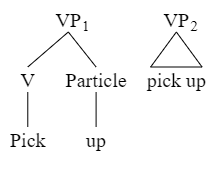
\includegraphics[width=1.13542in,height=\textheight]{Figures/syntax_tree.png}

}

\caption{\label{fig-lossinternalstructure}A diagram of two ways the word
\emph{pick up} could be stored. The left tree demonstrates a stored
representation of \emph{pick up}, where the internal structure is still
intact. The right tree demonstrates a holistically stored unit, where
there is a loss of internal structure. Note that both of these are
stored structures, as opposed to a compositional representation of
\emph{pick up} which would be comprised of the individual
representations \emph{pick} and \emph{up}.}

\end{figure}%

It's worth noting that in the case of phrasal verbs like \emph{pick up},
it can't be the case that the entire internal representation is lost
because it is possible to syntactically alternate it (e.g., \emph{pick
up the cup} vs \emph{pick the cup up}). However, it is possible that
semantic or lemma information is lost in the holistic representation.
That is, it is possible that syntactic and/or morphological information
may be preserved even if semantic or lemma information is lost. In other
words, loss of internal representation may happen at different levels as
opposed to being an all-or-nothing process.

\subsection{Present Study}\label{present-study}

The present study examines the factors that drive storage and the
representations of stored items by extending \citet{kapatsinski2009} to
look at the effects of both frequency, predictability, and their
interaction on the processing of V+\emph{up} phrases. Similar to
\citet{kapatsinski2009}, participants are tasked with pressing a button
once they hear the segment \emph{up} (which in our study occurs either
as a particle within verb phrases, e.g., \emph{pick up}, or part of a
word, e.g., \emph{puppet}), but in our case the stimuli varied in
frequency, predictability, and whether they were a phrasal verb or not.
Since both frequency and predictability effects are rather robust in the
literature, we should at the very least see a negative correlation
between frequency and predictability and recognition time (up to perhaps
a certain point, where recognition time may increase). Further, if
predictability is not a driving factor of storage, we should see an
increase in recognition times for only the most \emph{frequent} phrases.
On the other hand, if predictability does drive storage, we may see an
increase in reaction time for both frequent and predictable phrases.

\section{Methods}\label{methods}

\subsection{Participants}\label{participants}

Participants were recruited through the University of California, Davis
Linguistics/Psychology Human Subjects Pool. 350 people participated in
this study and were compensated in the form of course credit. All
participants self-reported being native English speakers. Additionally,
44 participants were excluded due to an accuracy score below our
threshold of 70\%, leaving a total of 306 participants for the data
analysis.

\subsection{Materials}\label{materials}

We searched the Google \emph{n}-grams corpus
\citep{linSyntacticAnnotationsGoogle2012} for the most predictable and
the highest frequency phrases that matched our criteria of containing a
verb immediately followed by the word \emph{up}. We operationalized
predictability as the odds ratio of the probability of \emph{up}
occurring immediately after the verb to the probability of any other
word occurring (Equation~\ref{eq-logodds}).

\begin{equation}\phantomsection\label{eq-logodds}{
\frac{\mathrm{count(\textit{Verb+up})}}{\mathrm{count(\textit{Verb})} - \mathrm{count(\textit{Verb+up})}} 
}\end{equation}

In non-mathematical terms, the above equation quantifies how likely
\emph{up} is to follow after the verb relative to every other word that
could follow. For example, the odds ratio of \emph{pick up} would be the
number of times the entire verb phrase occurs -- \emph{pick up} --
divided by the number of times the verb -- \emph{pick} -- occurs without
\emph{up} following it.

For the purposes of the present study, we gathered a variety of phrases
that varied in both their predictability and frequency and their
combination. In order to do this, we extracted the 50 most frequent
Verb+\emph{up} items and the 50 most predictable ones. Next, we selected
100 more by randomly sampling from the remaining items. In order to
ensure stable predictability estimates we eliminated words that a
college-aged speaker wouldn't have heard more than 10 times.\footnote{\citet{levyProcessingExtraposedStructures2012}
  extrapolated that the average college-aged speaker has heard about 350
  million words in their lifetime. Thus we excluded items that had a
  frequency smaller than 10 per 350 million.} We then visually inspected
the data to confirm that our data spanned across both the frequency and
predictability continuum. This distribution is presented in
Figure~\ref{fig-stimplot}.

\begin{figure}

\centering{

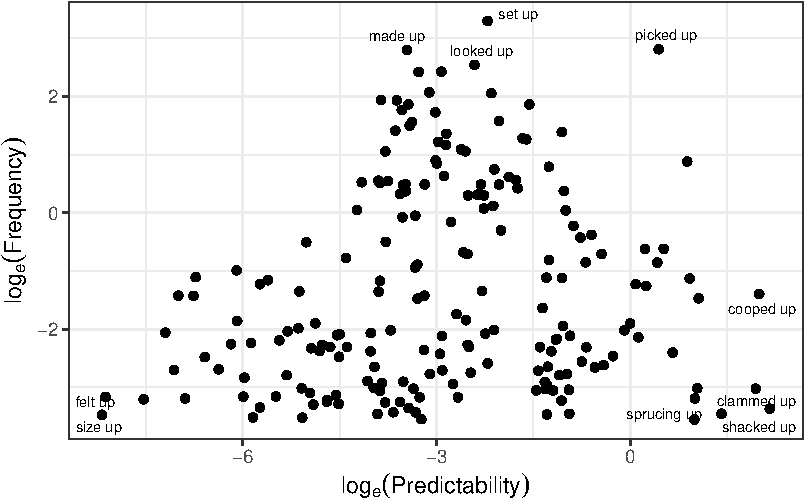
\includegraphics[width=0.8\textwidth,height=\textheight]{quarto-writeup_files/figure-pdf/fig-stimplot-1.pdf}

}

\caption{\label{fig-stimplot}log-predictability by log-frequency (per
million) plot of our items.}

\end{figure}%

Phrasal verbs show a syntactic alternation that is not present in all
verb+\emph{up} collocations (e.g., in the example below \emph{lightened
up the room} is fine, but \emph{lightened the room up} is weird at
best). It is possible that due to this syntactic alternation, phrasal
verbs may be stored regardless of frequency and predictability. This is
because in order to properly use phrasal verbs, a speaker must be aware
of the syntactic alternation, which can't simply be predicted
compositionally (e.g., some V+\emph{up} phrases are phrasal verbs, while
other V+\emph{up} phrases are not phrasal verbs\footnote{Note that this
  largely correlates with whether the verb is transitive or not.}).
Thus, we additionally coded our stimuli for whether they were phrasal
verbs or not. This coding was done based on whether they could
syntactically alternate between having the noun within the verb phrase
and having the noun immediately after the verb phrase. For example,
since both \emph{pick the cat up} and \emph{pick up the cat} are
grammatical, \emph{pick up} was classified as a phrasal verb. Each item
was checked by two of the authors. Disagreement was easily resolved by
discussion and an agreement was reached for every item.

\begin{exe} 
\ex
  \begin{xlist}
    \ex The student lightened up the room. \\
    \ex ??The student lightened the room up. \\
  \end{xlist}
\end{exe}

We also searched the same corpus for words that contained the segment
\emph{up} (e.g., \emph{cupcake}). In order to gather a subset of words
that roughly matches the frequency range of our experimental stimuli, we
extracted the 50 most frequent words, then sampled from the rest of the
dataset to gather an additional 100 words. These 350 items together
comprise our stimuli.

For each item, we constructed two sentences: one sentence which
contained \emph{up}, and one sentence that was identical except that it
didn't include the segment \emph{up.} For words, the entire word was
replaced. For phrases, \emph{up} was simply deleted if possible (e.g.,
\emph{clean up} replaced with \emph{clean}). If this resulted in an
awkward sentence, the entire phrase was replaced. An example is given
below.

\begin{exe} 
\ex
  \begin{xlist}
    \ex He picked up the phone and answered the call. \\
    \ex He grabbed the phone and answered the call. \\
  \end{xlist}
\end{exe}

In summary, our stimuli were comprised of 200 Verb+\emph{up} phrases
that varied in both frequency and predictability, 150 words that
contained \emph{up}, and 350 filler sentences which were matched with
our experimental sentences with the exception of having \emph{up}
replaced.

After creating the sentences, a native English speaker then recorded
each sentence in a random order to minimize any list effect. We
subsequently equalized the amplitude such that every sentence was
roughly the same loudness.

\subsection{Procedure}\label{procedure}

Participants were presented with audio sentences via Pavlovia
(\url{https://pavlovia.org/}), a website for presenting PsychoPy
experiments \citep{peircePsychoPy2ExperimentsBehavior2019}. Each
participant was presented with 3 practice trials and then 350 sentences.
While we had a total of 700 sentences, participants didn't see both the
filler and experimental sentence for the same item, thus they only saw
half of the stimuli. The order of the sentences was random and exactly
half of the sentences contained the target segment (to avoid biasing the
participants towards a specific response). Participants were instructed
to press a key as soon as they heard the segment \emph{up}, or to press
a separate key at the end of the sentence if they did not hear the
target segment in the sentence. We then recorded their reaction time of
the button press. The experiment took approximately 40 minutes.

\section{Results}\label{results}

The data\footnote{The stimuli, data, and analyses scripts can all be
  found freely available here:
  \url{https://github.com/znhoughton/Recognizability-Experiment}} was
analyzed using General Additive Mixed models, as implemented in the
\emph{mgcv} package \citep{mgcv} within the R programming environment
\citep{Rpackage}. General Additive Mixed Models are models that allow us
to model our outcome variable as a combination of the predictors. GAMMs
differ from generalized linear regression models in that they allow the
predictors to be modeled as non-linear functions, similar to polynomial
regression. Specifically, in a Generalized Additive Mixed Model,
beta-coefficients are replaced with a smooth function, which is a
combination of splines. The more splines that we include, the more
wiggly our line will be. In order to avoid overfitting, GAMMs also
include a penalty term, \(\lambda\), which can be modified to penalize
more wiggly lines that aren't justified by the data. While the
predictors are allowed to vary non-linearly, the linking function in our
case was linear (i.e., response time varied linearly with the spline
functions). Our decision to use GAMMs was driven by our hypothesis that
recognition times may vary non-linearly as a function of frequency
and/or predictability \citep[as suggested by][]{kapatsinski2009}.

For all of our models, the dependent variable was the time it took for
participants to react to the onset of the target segment in experimental
sentences/sentences containing \emph{up} (i.e., the time it took
participants to press the button after hearing \emph{up}).

In order to visualize the surface of the interaction effect between
frequency and predictability, we first ran a model with our independent
variable as the interaction between log-predictability and
log-frequency, which was allowed to vary non-linearly, and duration of
the segment, which was not allowed to vary non-linearly. Additionally,
we also included random intercepts for participant, trial, and item, as
well as random by-participant slopes for predictability, frequency,
their interaction, and trial. All our random-effects were allowed to be
wiggly (non-linear). Our model formula is included below in
Equation~\ref{eq-gamminteraction}. This model allows us to visualize the
surface of the interaction effect. Note that in GAMMs, the syntax
\texttt{ti()} is used to model the interaction effects since it produces
a tensor product interaction from which the main-effects have been
excluded. On the other hand \texttt{te()} models the full tensor product
smooth without the main-effects excluded. Thus when modeling the
main-effects with the interaction effect we use \texttt{ti()} and when
modeling the surface (that is, without separating the main-effects from
the interaction) we use \texttt{te()}.

\begin{equation}\phantomsection\label{eq-gamminteraction}{
\begin{aligned}log(RT) & \sim te(Predictability, Frequency) + Duration + s(participant, bs = \text{`}re\text{'}) + s(Item, bs = \text{`}re\text{'}) \\& + s(trial, bs = \text{`}re\text{'}) + s(Predictability, Frequency, participant, bs = \text{`}re\text{'}) \end{aligned}
}\end{equation}

The results of this model are presented in Table~\ref{tbl-gamModelTab}
and visualized in Figure~\ref{fig-gam2dplot1}. We found no significant
effect of the tensor product smooth.\footnote{We also examined the
  interaction between frequency and predictability on accuracy (whether
  they correctly responded to whether \emph{up} was present in the
  sentence) and similarly found no significant effect.} Although the
tensor product smooth for the interaction effect was not significant,
it's possible that the frequency or predictability independently affect
recognition times. Thus, we ran an additional Generalized Additive Model
with log-frequency, log-predictability, and the interaction between
log-frequency and log-predictability as fixed-effects that could vary
non-linearly. Similar to before, duration of the segment was also
modeled as a fixed-effect that could not vary non-linearly. The
random-effects structure for this model was identical to the previous
two models. The model syntax is included below in
Equation~\ref{eq-gammFull}:

\begin{equation}\phantomsection\label{eq-gammFull}{
\begin{aligned}log(RT) & \sim ti(Predictability) + ti(Frequency) + ti(Predictability, Frequency) + Duration \\ & + s(participant, bs = \text{`}re\text{'}) + s(Item, bs = \text{`}re\text{'})  + s(trial, bs = \text{`}re\text{'}) \\ & + s(Predictability, Frequency, Trial, Participant, bs = \text{`}re\text{'}) \end{aligned}
}\end{equation}

Our results are presented in Table~\ref{tbl-gamModelInterTab};
Equation~\ref{eq-gammFull} and visualized in
Figure~\ref{fig-gammodelinterplot}. The results demonstrated a
significant main-effect of predictability (\emph{p} \textless{} 0.05),
but no significant effect of frequency (\emph{p} = 0.327).\footnote{We
  ran a follow-up model without the interaction to determine whether
  including the interaction effect takes away our power to detect an
  effect of frequency, however the results for our main-effects are
  consistent regardless of whether we include the interaction between
  frequency and predictability in the model.}

To summarize the results of our generalized additive models, we found no
interaction effect between frequency and predictability, no main effect
of frequency, but we do find a significant main effect of
predictability.

In the Psycholinguistics literature, generalized additive mixed models
are not yet well established. Thus, we ran a follow-up Bayesian
quadratic regression model to further examine the effects of frequency
and predictability on recognition times. Since the Generalized Additive
Model suggested that there was no significant interaction between
frequency and predictability, we left out the interaction term from the
regression model. The random-effects were modeled without correlations
between them in order to allow the model to run faster.
Equation~\ref{eq-BayesianFullModelSyntax} below presents the full model
syntax:

\begin{equation}\phantomsection\label{eq-BayesianFullModelSyntax}{
\begin{aligned}
log(RT) & \sim  log(Frequency) + log(Predictability) + Duration + log(Frequency)^2  + log(Predictability)^2 \\ & + (1 + log(Frequency) + log(Predictability) + log(Frequency^2) + log(Predictability^2) \\& + Duration || Participant) + (1 || Item)
\end{aligned}
}\end{equation}

The results of this model are presented in
Table~\ref{tbl-brmsQuadraticNoInter} and visualized in
Figure~\ref{fig-FullQuadraticPlot}. Following
\citet{houghtonTaskdependentConsequencesDisfluency2023}, in some cases
where the credible interval crosses zero, we also report the percentage
of posterior samples greater than or less than zero. For the current
model, although the credible intervals for both quadratic terms crossed
zero, nearly 97\% of the posterior samples for predictability\(^2\) were
greater than zero, and nearly 93\% of the posterior samples for
frequency\(^2\) were greater than zero. A plot of the posterior
distribution for each coefficient is presented in
Figure~\ref{fig-posteriorplotFullQuadratic}. The results suggest a
U-shaped effect of predictability and a marginal u-shaped effect of
frequency on recognition times. In other words, participants recognized
\emph{up} faster as frequency or predictability increased, except for
the most frequent or most predictable items, where participants were
slower to recognize \emph{up}.

Finally, we replicated the analyses from \citet{kapatsinski2009} using
two Bayesian quadratic regression models \citep[implemented in
\emph{brms;}][]{brms}, one which only included frequency, and one which
only included predictability. For the frequency model, the fixed-effects
were log-frequency and log-frequency\(^2\), along with duration. The
model also included random intercepts for participant and item, and
random slopes for log-frequency by participant, duration by participant,
and log-frequency\(^2\) by participant.

The quadratic regression with predictability was identical to the
quadratic regression with frequency, except that log-frequency was
replaced with log-predictability, and log-frequency\(^2\) was replaced
with log-predictability\(^2\). The random-effects were modeled without
correlations between them for both models (this was done to allow the
model to run faster, since we collected a large amount of data).

The model syntax for both models is included below in
Equation~\ref{eq-brmsFreq} and Equation~\ref{eq-brmsPredic}:

\begin{equation}\phantomsection\label{eq-brmsFreq}{
\begin{aligned}
log(RT) & \sim log(Frequency) + Duration + log(Frequency)^2 \\ & + (1 + log(Frequency) + log(Frequency)^2 + Duration || Participant) + (1 || Item)
\end{aligned}
}\end{equation}

\begin{equation}\phantomsection\label{eq-brmsPredic}{
\begin{aligned}
log(RT) & \sim log(Predictability) + Duration + log(Predictability)^2 \\ & + (1 + log(Predictability) + log(Predictability)^2 + Duration || Participant) + (1 || Item)
\end{aligned}
}\end{equation}

The results of our first model are presented in
Table~\ref{tbl-brmsFreq}. While the credible interval for
log(frequency)\(^2\) crosses zero, over 95\% of the posterior samples
were greater than zero, suggesting an effect of frequency\(^2\) on
recognition times. A visualization of the model predictions is presented
in Figure~\ref{fig-FreqOnlyPlot} and a visualization of the posterior
distribution is presented in Figure~\ref{fig-FreqOnlyBetaPlot}.

The results of our second model are presented in
Table~\ref{tbl-brmsPredic}. While the credible interval for
log(predictability)\(^2\) crosses zero, over 96\% of the posterior
samples were greater than zero, suggesting a meaningful effect. A
visualization of the model predictions is included in
Figure~\ref{fig-PredicOnlyPlot} and a visualization of the posterior
distribution is presented in Figure~\ref{fig-PredicOnlyBetaPlot}.

In summary, our results suggest that when considered independently,
there appears to be a U-shaped effect for both frequency and
predictability. The effect for frequency is not as reliably detected
when predictability is also accounted for in our models, however we do
find weak evidence for it. We do not find strong evidence for an
interaction between frequency and predictability but it is possible that
our study simply does not have the power to detect an interaction
effect.

\begin{table}

\caption{\label{tbl-gamModelTab}Model results for the generalized
Additive Mixed Model cotanining only the interaction between frequency
and predictability.}

\centering{

\begin{tabular}{lrrrl}
\toprule
  & edf & Ref.df & F & p-value\\
\midrule
te(log-predictability, log-frequency) & 5.59 & 5.73 & 1.86 & 0.090\\
s(trial) & 0.99 & 1.00 & 115.38 & <0.001\\
s(participant) & 296.00 & 305.00 & 39.74 & <0.001\\
s(item) & 175.44 & 195.00 & 10.68 & <0.001\\
s(log-predictability, log-frequency, trial, participant) & 43.00 & 306.00 & 0.46 & 0.100\\
\bottomrule
\end{tabular}

}

\end{table}%

\begin{table}

\caption{\label{tbl-gamModelInterTab}Model results for the Generalized
Additive Mixed Model cotaining Frequency, Predictability, and the
interaction between them.}

\centering{

\begin{tabular}{lrrrl}
\toprule
  & edf & Ref.df & F & p-value\\
\midrule
ti(log-frequency) & 2.16 & 2.20 & 1.73 & 0.270\\
ti(log-predictability) & 1.97 & 2.01 & 4.10 & 0.020\\
ti(log-frequency, log-predictability) & 1.00 & 1.00 & 0.89 & 0.350\\
s(participant) & 296.33 & 305.00 & 37.72 & <0.001\\
s(item) & 175.70 & 195.00 & 10.76 & <0.001\\
\addlinespace
s(log-predictability, log-frequency, participant) & 0.17 & 305.00 & 0.00 & 0.600\\
\bottomrule
\end{tabular}

}

\end{table}%

\begin{table}

\caption{\label{tbl-brmsFreq}Results for the Bayesian quadratic
regression model containing only frequency and frequency\(^2\).}

\centering{

\begin{tabular}{lllllr}
\toprule
  & Estimate & Est.Error & Q2.5 & Q97.5 & \% Samples > 0\\
\midrule
Intercept & -0.102 & 0.025 & -0.150 & -0.054 & 0.000\\
log-frequency & 0.016 & 0.011 & -0.005 & 0.038 & 93.310\\
Duration & -0.084 & 0.098 & -0.274 & 0.108 & 19.355\\
log-frequency\textasciicircum{}2 & 0.006 & 0.004 & -0.001 & 0.013 & 95.225\\
\bottomrule
\end{tabular}

}

\end{table}%

\begin{table}

\caption{\label{tbl-brmsPredic}Results for the Bayesian quadratic
regression model containing only predidctability and
predictability\(^2\).}

\centering{

\begin{tabular}{lllllr}
\toprule
  & Estimate & Est.Error & Q2.5 & Q97.5 & \% Samples > 0\\
\midrule
Intercept & -0.110 & 0.027 & -0.163 & -0.058 & 0.0000\\
log-predictability & 0.008 & 0.011 & -0.014 & 0.029 & 75.7350\\
Duration & -0.089 & 0.098 & -0.280 & 0.102 & 18.4225\\
log-predictability\textasciicircum{}2 & 0.003 & 0.002 & -0.000 & 0.006 & 96.0975\\
\bottomrule
\end{tabular}

}

\end{table}%

\begin{table}

\caption{\label{tbl-brmsQuadraticNoInter}Model results for the Bayesian
quadratic regression model containing fixed-effects for frequency,
predictability, and their quadratics.}

\centering{

\begin{tabular}{lllllr}
\toprule
  & Estimate & Est.Error & Q2.5 & Q97.5 & \% Samples > 0\\
\midrule
Intercept & -0.102 & 0.029 & -0.161 & -0.046 & 0.02625\\
log-frequency & 0.019 & 0.011 & -0.002 & 0.041 & 96.15625\\
log-predictability & 0.009 & 0.011 & -0.013 & 0.032 & 78.99750\\
duration & -0.135 & 0.098 & -0.328 & 0.057 & 8.27125\\
log-predictability\textasciicircum{}2 & 0.003 & 0.002 & -0.000 & 0.007 & 96.88125\\
\addlinespace
log-frequency\textasciicircum{}2 & 0.005 & 0.004 & -0.002 & 0.012 & 92.94375\\
\bottomrule
\end{tabular}

}

\end{table}%

\begin{figure}

\centering{

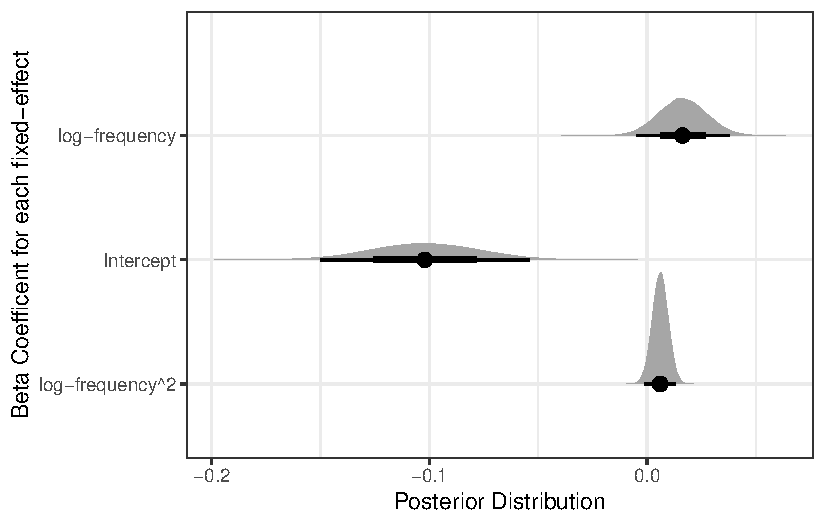
\includegraphics[width=0.8\textwidth,height=\textheight]{quarto-writeup_files/figure-pdf/fig-FreqOnlyBetaPlot-1.pdf}

}

\caption{\label{fig-FreqOnlyBetaPlot}Plot of the posterior distribution
for the beta value of each fixed-effect in our frequency-only quadratic
regression model. The y-axis contains the different fixed-effects and
the x-axis contains the posterior distribution of beta values for the
corresponding fixed-effect.}

\end{figure}%

\begin{figure}

\centering{

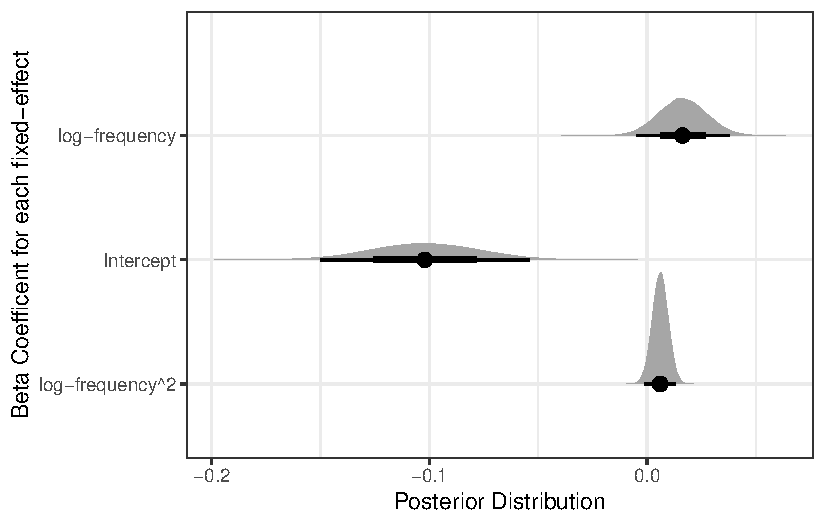
\includegraphics[width=0.8\textwidth,height=\textheight]{quarto-writeup_files/figure-pdf/fig-PredicOnlyBetaPlot-1.pdf}

}

\caption{\label{fig-PredicOnlyBetaPlot}Plot of the posterior
distribution for the beta value of each fixed-effect in our
predictability-only quadratic regression model. The y-axis contains the
different fixed-effects and the x-axis contains the posterior
distribution of beta values for the corresponding fixed-effect.}

\end{figure}%

\begin{figure}

\centering{

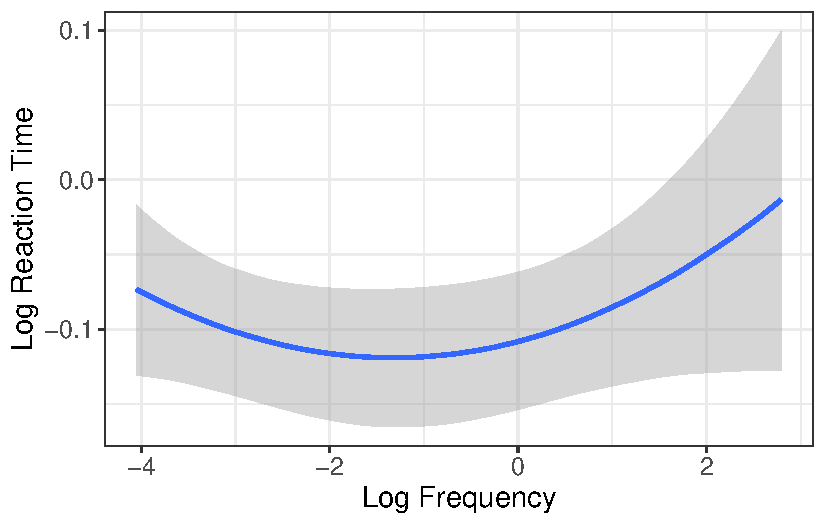
\includegraphics[width=0.6\textwidth,height=\textheight]{quarto-writeup_files/figure-pdf/fig-FreqOnlyPlot-1.pdf}

}

\caption{\label{fig-FreqOnlyPlot}Model predictions for the effects of
frequency on reaction times for the frequency-only Bayesian quadratic
model.}

\end{figure}%

\begin{figure}

\centering{

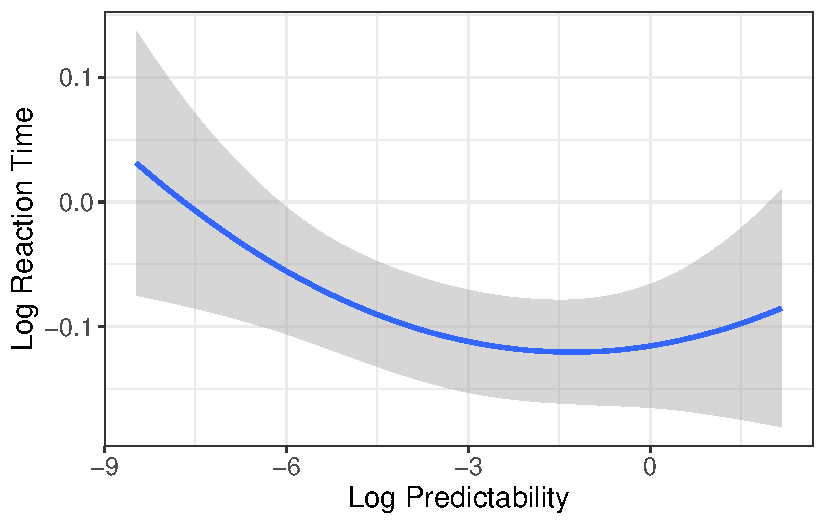
\includegraphics[width=0.6\textwidth,height=\textheight]{quarto-writeup_files/figure-pdf/fig-PredicOnlyPlot-1.pdf}

}

\caption{\label{fig-PredicOnlyPlot}Model predictions for the effect of
predictability on reaction times for the predictability-only models.}

\end{figure}%

\begin{figure}

\centering{

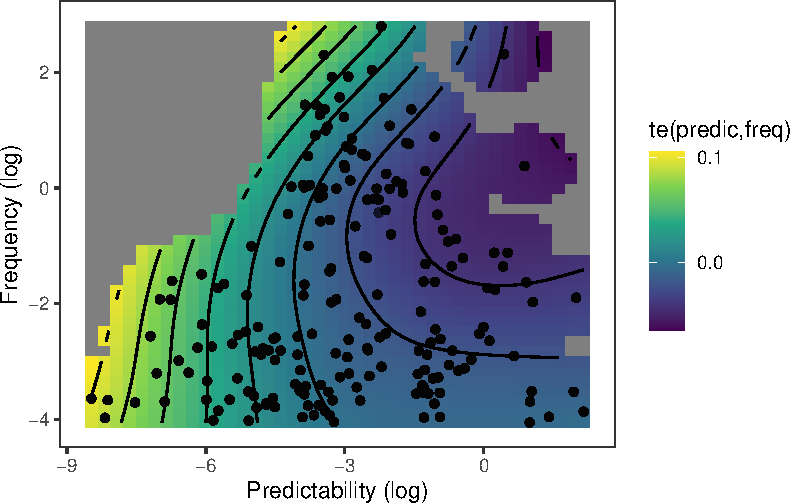
\includegraphics[width=0.8\textwidth,height=\textheight]{quarto-writeup_files/figure-pdf/fig-gam2dplot1-1.pdf}

}

\caption{\label{fig-gam2dplot1}Plot of the interaction effect between
predictability and frequency of our GAM model containing only the
interaction between frequency and predictability. The brightness of the
coloration denotes the strength of the effect at the point in the graph.
Brighter colors denote longer reaction times.}

\end{figure}%

\begin{figure}

\centering{

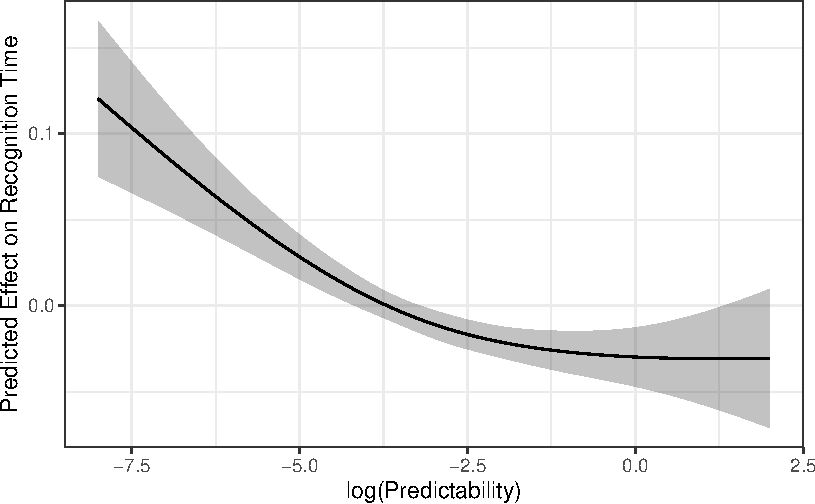
\includegraphics{quarto-writeup_files/figure-pdf/fig-gammodelinterplot-1.pdf}

}

\caption{\label{fig-gammodelinterplot}Plot of our GAM model's predicted
effect of log(predictability) on recognition time.}

\end{figure}%

\begin{figure}

\centering{

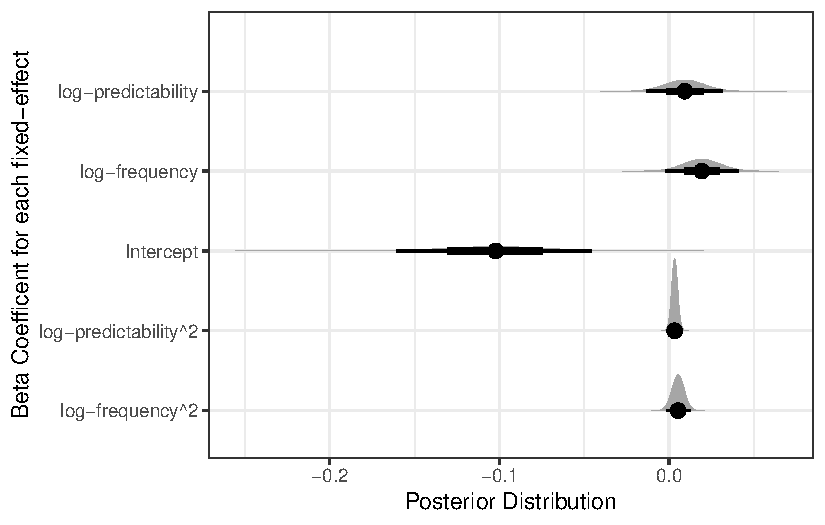
\includegraphics[width=0.8\textwidth,height=\textheight]{quarto-writeup_files/figure-pdf/fig-posteriorplotFullQuadratic-1.pdf}

}

\caption{\label{fig-posteriorplotFullQuadratic}Plot of the posterior
distribution for the beta value of each fixed-effect in our Bayesian
quadratic regression model. The y-axis contains the different
fixed-effects and the x-axis contains the posterior distribution of beta
values for the corresponding fixed-effect.}

\end{figure}%

\begin{figure}

\centering{

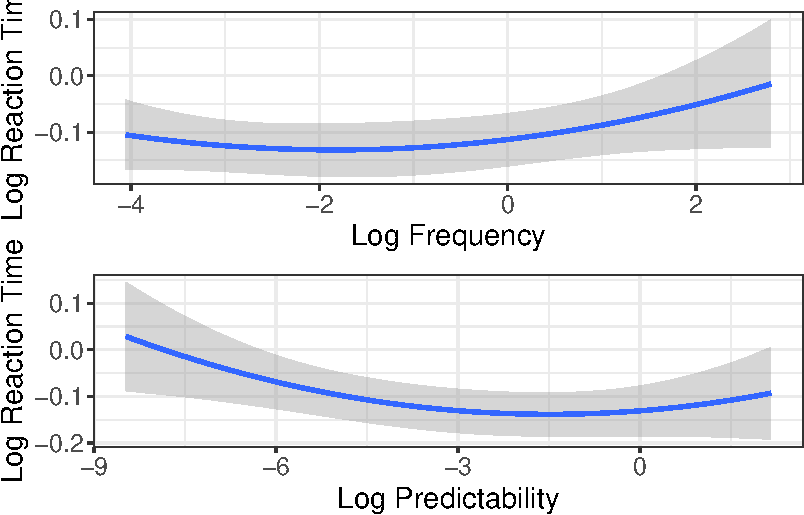
\includegraphics[width=0.8\textwidth,height=\textheight]{quarto-writeup_files/figure-pdf/fig-FullQuadraticPlot-1.pdf}

}

\caption{\label{fig-FullQuadraticPlot}Visualization of the model results
from Table~\ref{tbl-brmsQuadraticNoInter} for frequency (top) and
predictability (bottom). Frequencies are per million.}

\end{figure}%

\section{Discussion}\label{discussion}

The present study examined the effects of frequency and predictability
on the recognizability of the particle \emph{up} in English phrasal
verbs. We found a U-shaped effect for both frequency and predictability
on recognizability: as frequency and predictability increased, people
were faster at recognizing \emph{up}, until reaching the highest
frequency/most predictable items, where people were slower.
Additionally, we also found no meaningful differences between phrasal
verbs (e.g., \emph{pick up}) and non-phrasal verbs (e.g., \emph{stir
up}), suggesting that this slowdown is due to statistical properties of
the language as opposed to syntactic properties.

There are three possible accounts for the slowdown we see for the
highest frequency or predictability items. First, it's possible that
people are attending less to \emph{up} or even skipping it in high
frequency and high predictability phrases. This account, unlike the
other accounts that we'll discuss, does not explicitly require the high
frequency and high predictability phrases to be stored. Instead, the
listener may be able to process the meaning of the phrase fast enough
that they don't need to wait to hear the entire phrase. For example,
it's possible that for high-frequency and high-predictability items,
when accessing the first word, e.g., \emph{pick}, the listener accesses
the representation of the entire phrase --- either a holistic
representation or a compositional representation --- immediately, before
even hearing \emph{up}. The listener can then continue to process the
next words (skipping over \emph{up}). Since the task is to respond when
they hear \emph{up}, the delay in reaction time may be because they're
not accessing the phonological representation of \emph{up}. Instead,
they may access the semantic representation of the phrase without
initially accessing the phonological representation of \emph{up} and go
on to recover the phonological representation from the semantic
representation of the phrase, causing a delay in recognition time.
Indeed, this possibility was suggested by \citet{healy1976}, who
suggested that in reading once people process the meaning of a word,
they move on to the next word regardless of whether they have processed
each individual letter. This account doesn't explicitly require
\emph{pick up} to be stored holistically since a listener could hear
\emph{pick}, predict \emph{up}, and compose the meaning \emph{pick up}
despite having not heard \emph{up}. However, it also isn't incompatible
with a storage account, since the listener might hear \emph{pick,}
predict \emph{up}, and then accesses a stored holistic representation of
\emph{pick up}. In other words, if listeners are attending less to
\emph{up}, then it's unclear whether the listeners are accessing a
representation formed by a compositional process (i.e., accessing
\emph{pick,} predicting \emph{up,} and composing \emph{pick up}) or
simply retrieving a stored form from memory (accessing a holistic
representation \emph{pick up}).

The next two accounts all require the high-frequency and
high-predictability items to be stored holistically, but vary with
respect to whether the holistically stored representations retain their
internal structure.

It is possible that the slowdown for the high frequency and high
predictability items is due to competition between an additional
representation. This competition can either be between a holistic
representation that has internal structure and a compositional
representation, or between a holistic representation that does not have
internal structure and the compositional representation. Compositional
representation here refers to a representation that is formed by
accessing individual forms (e.g., \emph{pick} and \emph{up}) and
combining them via some generative process. High-frequency and
high-predictability items may develop a holistic representation separate
from the compositional representation and this additional representation
may compete with the compositional representation causing the slowdown.
This account doesn't necessarily need to involve a loss of internal
structure because simply having an additional representation to compete
with can result in a slowdown, however it also not incompatible with an
account where the holistic representation has lost some of its internal
structure. These two possibilities both account for the slowdown at the
highest frequency and highest predictability items.

To break it down further, there is a good deal of evidence that
different mental representations compete for recognition
\citetext{\citealp{oppenheimLexicalCompetitionDemand2019}; \citealp[c.f.][]{staubInfluenceClozeProbability2015}}.
A representation is selected once it receives sufficiently more
activation than its competitors
\citep{mcclellandInteractiveActivationModel1981}. For example, in
picture-naming tasks in which participants are tasked with naming a
picture while confronted with a distractor word, participants are
generally slower to produce the intended word when the distractor word
is semantically related to the picture
\citep{starreveldSemanticInterferenceOrthographic1995, schriefersExploringTimeCourse1990, mcclellandInteractiveActivationModel1981}.
This effect is not restricted to production as we see similar
competition effects in comprehension as well. For example,
\citet{magnuson2007} examined the role of competition in word
recognition using a visual world paradigm, where participants saw words
on a screen and were instructed to select the word that they heard. To
measure word-recognition, an eye-tracker was used to track pupil
fixations. In each of the trials there was a single distractor image.
They found that words with low cohort density (i.e., words that have
fewer phonological competitors) showed a larger proportion of target to
nontarget fixations. That is, participants looked the distractor image
less relative to the target word when the word had fewer competitors.
Given the inhibitory effects of competition, it is possible that the
delay in reaction time for \emph{up} in high-frequency and
predictability phrases may be a consequence of an additional
representation competing with the compositional representation. However,
there is also evidence that competition has no effect on comprehension
\citep{staubInfluenceClozeProbability2015}. Using reaction time data
from a cloze completion task, \citet{staubInfluenceClozeProbability2015}
demonstrated that a RACE model with neither facilitation nor inhibition
between competitors can account for the data. Thus the evidence for
competition effects in comprehension is mixed. Note that this account is
agnostic about whether the holistic representation has lost its internal
structure or not: simply having an additional representation to compete
with can cause the slowdown.

Lastly it is possible that rather than being driven by competition,
listeners are simply accessing a holistically stored representation of
the phrase that lacks internal structure. This interpretation seems
quite likely given that we see a U-shaped effect in both phrasal (e.g.,
\emph{pick up}) and non-phrasal verbs (e.g., \emph{stir up}). Phrasal
verbs have a syntactic alternation that may lead to all of them being
stored, regardless of whether they are frequent/predictable or not. For
example, In a corpus study, \citet{hampeTransitivePhrasalVerbs2012}
argued that \emph{Verb-Object-Particle} constructions and
\emph{Verb-Particle-Object} constructions are two distinct
constructions.\footnote{However, the same study also makes the claim
  that these templates are different from more lexically specific
  constructions, thus it is unclear in what ways these templates may
  pattern similarly to holistically stored lexical items.} If the
increase in reaction time is simply due to competition between the
holistically stored representation and the individual word-level
representations, then if all phrasal verbs are stored we would expect
all of the phrasal verbs to be recognized more slowly. This is because
all of the phrasal verbs, regardless of frequency, would have an
additional representation that would compete for activation. However, we
only see a slowdown for the most frequent or most predictable phrases,
suggesting that storage alone isn't driving the effect. Instead, it is
the combination of storage and usage that leads to loss of internal
representation.

One explanation for why high frequency and high predictability items may
not have an intact internal representation is that the internal
structure for those items may never have been learned to begin with.
Children are experts at statistical learning and use transitional
probabilities to divide the continuous speech stream
\citep{saffran1996}. High predictability phrases in the present study,
by definition, have higher transitional probabilities between words.
Thus if children are relying on transitional probabilities to separate
speech into individual words, the individual words in the most
predictable phrases may not be separated out of the speech stream
initially.

Further, many high-frequency (e.g., \emph{set up}) and
high-predictability (e.g., \emph{conjure up}) phrases have semantically
vague relationships that might make it difficult to split them up on a
semantic basis. It seems plausible then that maybe these phrases weren't
learned as being composed of individual words initially and thus the
internal structure for the holistically stored items may not have been
learned. The example, \emph{trick or treat}, is a prime example of a
phrase that does not seem to have a clear semantic relationship between
the phrase and its component parts.

On the other hand, the internal structure may have been lost over time.
For example, \citet{harmonPuttingOldTools2017} demonstrated that as
learners repeatedly experience a form with a specific meaning, they
become more likely to use that form to express novel meanings in
production (resulting in semantic extension). It is possible that this
accessibility effect similarly drives a loss of internal structure: As a
phrase becomes more semantically extended, the internal structure may be
lost over time. That is, as a phrase such as \emph{pick up} becomes
extended to express novel meanings such as \emph{continue} (``Let's pick
up from where we last left off''), the relationship between the phrase
and its internal pieces (e.g., the relationship between \emph{pick up}
and the individual words \emph{pick} and \emph{up}) becomes less
transparent, and the learner may slowly unlearn this relationship as it
becomes less useful.

In summary, our results suggest that both frequency and predictability
may drive the holistic storage of phrasal verbs, and these holistically
stored items may compete with their component parts during lexical
access. However, future work is still needed to confirm whether the
slowdown for the highest frequency and highest predictability items is
indeed due to a stored holistic representation or if it's due to
shallower attention mechanisms.

\section{Acknowledgements}\label{acknowledgements}

The authors would like to thank Dingyi (Penny) Pan for reading and
offering comments on a draft of this paper. The authors would also like
to thank Vsevolod Kapatsinski and Zara Harmon for providing helpful
discussion about the nature of competition in lexical processing.

\newpage


  \bibliography{r-references.bib,references.bib}



\end{document}
